\documentclass[10pt,twocolumn,letterpaper]{article}

% ---------------------------------------------------------------
% Include basic CVPR package in rebuttal mode

\usepackage[rebuttal]{cvpr}

% ---------------------------------------------------------------
% Other packages

% Commonly used abbreviations (\eg, \ie, \etc, \cf, \etal, etc.)
\usepackage{eccvabbrv}

% Include other packages here, before hyperref.
\usepackage{graphicx}
\usepackage{booktabs}
\usepackage[table]{xcolor}

% The "axessiblity" package can be found at: https://ctan.org/pkg/axessibility?lang=en
\usepackage[accsupp]{axessibility}  % Improves PDF readability for those with disabilities.


% ---------------------------------------------------------------
% Hyperref package
% If you comment hyperref and then uncomment it, you should delete
% egpaper.aux before re-running latex.  (Or just hit 'q' on the first latex
% run, let it finish, and you should be clear).

\definecolor{eccvblue}{rgb}{0.12,0.49,0.85}
\usepackage[pagebackref,breaklinks,colorlinks,citecolor=eccvblue]{hyperref}


% ---------------------------------------------------------------
% If you wish to avoid re-using figure, table, and equation numbers from
% the main paper, please uncomment the following and change the numbers
% appropriately.
%\setcounter{figure}{2}
%\setcounter{table}{1}
%\setcounter{equation}{2}

% If you wish to avoid re-using reference numbers from the main paper,
% please uncomment the following and change the counter for `enumiv' to
% the number of references you have in the main paper (here, 6).
%\let\oldthebibliography=\thebibliography
%\let\oldendthebibliography=\endthebibliography
%\renewenvironment{thebibliography}[1]{%
%     \oldthebibliography{#1}%
%     \setcounter{enumiv}{6}%
%}{\oldendthebibliography}


% ---------------------------------------------------------------
% TODO REBUTTAL: Please enter paper ID
\def\paperID{11591} % *** Enter the paper ID here
\def\confName{ECCV}
\def\confYear{2026}

\definecolor{MyCyan}{RGB}{0,163,218}
\definecolor{MyDarkBlue}{RGB}{0,103,165}
\definecolor{MyDarkGreen}{RGB}{56,116,51}
\definecolor{MyOrange}{RGB}{225, 95, 0}
\definecolor{MyMagenta}{RGB}{200,18,126}

\def\Ra{\textcolor{MyMagenta}{\textbf{SaV6}}\xspace}
\def\Rb{\textcolor{MyOrange}{\textbf{bfPP}}\xspace}
\def\Rc{\textcolor{MyCyan}{\textbf{xCve}}\xspace}
\renewcommand{\thetable}{R}

\begin{document}

% ---------------------------------------------------------------
% TODO REBUTTAL: Please enter paper title
\title{\LaTeX\ Guidelines for Author Response}  % **** Enter the paper title here

% \maketitle
\thispagestyle{empty}
\appendix


\noindent We thank the reviewers for valuable feedback, which will be incorporated.
%
They recognize our clear motivation (\Ra, \Rc) for this crucial problem (\Rb), and commend the intuitive decoupling of local compression from global reasoning (\Rb, \Rc).
%
Praised as a \emph{good idea} (\Ra, \Rc), our SVLM compressor yields strong performance across broad benchmarks, validated by thorough ablations (\Ra, \Rb).

\begin{table}[h]
    \vspace{-2em}
    \centering
    \setlength{\tabcolsep}{4pt} 
    \renewcommand{\arraystretch}{0.6}
    \caption{
        \textbf{Lat. \& Mem. on LVBench (1$\times$H100).} \textbf{Lat. V/L/O}: Vision Encoding \& Compression/LLM/Overall average latency (s). \textbf{Mem.}: Peak GPU Memory (GB). 
        %
        \protect\colorbox{green!15}{Green}: official default configs. Tokens: visual tokens before LLM.
        % (XComp compresses 16K$\to$1K within LLM). 
        \textbf{Analysis}: Baselines (DyToK, HoliTom, DyCoke) OOM at 128--512 frames, failing hour-long videos. \protect\colorbox{yellow!15}{Yellow} indicates matched frames solely for fair comparison (Tempo's $\leq$16 tok./frame prevents reaching 8K tokens for parity).
        %
        Similarly, \protect\colorbox{blue!10}{Blue} matches frames against specialized long video MLLMs.
    }
    \label{tab:latency_rebuttal}
    \resizebox{\linewidth}{!}{
    \begin{tabular}{l ccccccc}
        \toprule
        \textbf{Model} & \textbf{Frames} &\textbf{Tokens} & \textbf{Lat. V} & \textbf{Lat. L} & \textbf{Lat. O} & \textbf{Mem.} & \textbf{Accuracy} \\
        \midrule
                           Tempo, 6B   & 32     & $\leq$ 512  & 0.09 & 0.22 & 0.31 & 12.3 & 39.4 \\
        \rowcolor{green!15} DyCoke, 7B  & 32     & 2979       & 0.21 & 0.17 & 0.38 & 19.1 & 37.2 \\
        \rowcolor{green!15} HoliTom, 7B & 32     & 1568       & 0.25 & 0.13 & 0.37 & 17.9 & 38.5 \\
        \rowcolor{green!15} DyTok, 7B   & 32     & 4704       & 0.45 & 0.24 & 0.69 & 33.1 & 38.9 \\
        \rowcolor{green!15} XComp, 2B   & 2048   & 16384      & 30.0 & 2.05 & 32.0 & 21.3 & 46.2 \\
        \rowcolor{green!15} VideoChat-Flash, 7B  & 512 & 8192 & 1.20 & 0.35 & 1.55 & 25.6 & 48.2 \\
                           Tempo, 6B    & 512    & $\leq$ 8192& 1.06 & 0.28 & 1.34 & 24.5 & 50.5 \\
        \midrule
        \rowcolor{blue!10} Tempo, 6B    & 1024   & $\leq$ 8192& \textbf{2.04} & \textbf{0.27} & \textbf{2.31} & 37.5 & \textbf{52.3} \\
        \rowcolor{blue!10} VideoChat-Flash, 7B   & 1024 & 16384 & 2.39 & 0.73 & 3.12 & 35.9 & 47.4 \\
        \rowcolor{blue!10} XComp w/o QC, 2B      & 1024 & 16384 & 2.40 & 0.33 & 2.73 & \textbf{11.3} & 44.3 \\
        \midrule
        \rowcolor{yellow!15} Tempo, 6B      & 128    & $\leq$ 2048 & \textbf{0.28} & \textbf{0.22} & \textbf{0.50} & \textbf{14.8} & \textbf{42.7} \\
        \rowcolor{yellow!15} DyCoke, 7B     & 128    & 8154        & 0.82 & 0.46 & 1.28 & 29.8 & 41.1 \\
        \rowcolor{yellow!15} HoliTom, 7B    & 128    & 8780        & 1.10 & 0.66 & 1.77 & 32.8 & 41.8 \\
        \bottomrule
    \end{tabular}
    }
    \label{tab:rebuttal}
\end{table}
% -------------------------------------------------------

\vspace{-1.5em}
\noindent{\textcolor{MyMagenta}{\Large\textbf{------------\quad}}}
\textcolor{MyMagenta}{\textbf{Reviewer SaV6}} 
\textcolor{MyMagenta}{\Large\textbf{\quad---------------}}

% ----------------------------------------------------
%                      4/4
% ----------------------------------------------------
% Justification:
% 1. The submission can be stronger if the results are benchmarked against alternative SoTA compression strategies, specifically wavelet-based methods and latent self-pruning methods (e.g., XComp). Comparing TEMPO's training-heavy approach to these training-free or internal-pruning alternatives would better justify its architectural complexity. Also, publishing latency numbers and computational overhead (FLOPs) are essential to clarify the actual efficiency gains of SVLM and help us understand the trade-off between its reduced token budget and sequential processing costs.
% ----------------------------------------------------
% Suggestions For Rebuttal:
% 1. Performance Comparison: Provide a direct comparison of the SCORE model against the performance of token compression models based on wavelet/frequency domains, such as Wave-ViT (Yao et al., ECCV 2022), or latent self pruning methods, such as XComp (Zheyu Zhang et al., NeurIPS 2025). If there are newer models that authors become aware in these areas, use those models for comparison.
% 2. Publish latency numbers and computational overhead (FLOPs). This data would clarify the actual efficiency gains and help us understand the trade-off between the model's reduced token budget and its sequential processing costs.
% ----------------------------------------------------
% Summary for Reviewer's Expect:
% Compare to wavelet-based methods (Wave-ViT) and latent self-pruning methods (XComp). 
% Report latency and FLOPs.
% ----------------------------------------------------

\vspace{-0.2em}
\noindent{\textcolor{MyMagenta}{\textbf{Q1: Baselines.}}}
% ----------------------------------------------------
% W1:
% The papers completely misses some of the key works in video token compression, e.g., frequency or wavelet information based methods such as WaveVIT (Yao et al., ECCV 2022) or latent self-pruning methods such as XComp (Zheyu Zhang et al., NeurIPS 2025). Both of these methods are powerful as they don’t require an external models (like SCORE) to achieve token compression. This key insight is missing from the paper entirely.
% ----------------------------------------------------
% W2:
% Wavelet-based methods are training-free, allowing them to be applied to any LLM easily without significant distribution shift. Similarly, self-pruning methods use the latent space of the model itself to achieve extreme compression of one token per frame without needing additional training. In contrast, TEMPO requires training, especially for adaptation to new query patterns and out-of-distribution videos.
% ----------------------------------------------------
We prioritize wall-clock latency and peak memory over FLOPs. FLOPs correlate poorly with actual efficiency given cross-architecture differences, attention optimizations, and TEMPO's dynamic sequence lengths. For hour-long videos, latency and OOM limits are the definitive deployment bottlenecks.
% Since they prune with the LLM's attention, 
\textbf{1) Latent Self-Pruning (Tab.~\ref{tab:rebuttal}):} We evaluate DyCoke, DyToK, XComp, and V.C.-Flash. Since they prune \textit{within} the LLM's latent space, early layers still ingest massive tokens, triggering \textbf{Attention Dilution} and high latency for long videos. Conversely, Tempo compresses segments independently \textit{pre-LLM}, shielding the LLM from massive tokens.
%
\textbf{2) XComp's} QC-Comp requires multiple LLM forward passes, causing 30s vision latency (Lat. V) for long videos. Even without QC-Comp, when processing matched 1024 frames, XComp's intra-LLM pruning (16K $\rightarrow$ 1K) remains slower than Tempo due to massive token burdens in early layers.
%
\textbf{3) Wavelet-based Methods} target \textit{spatial} redundancy, whereas long videos bottleneck on extreme \textit{temporal} redundancy. To our knowledge, no wavelet-based long video MLLMs exist to report.


\vspace{-0.2em}
\noindent{\textcolor{MyMagenta}{\textbf{Q2: Error Analysis.}}}
% ----------------------------------------------------
% W1:
% Error Analysis and Failure cases, demonstrate qualitatively where the model has failed and what can be the potential root causes for the same.
% ----------------------------------------------------
% W2:
% The paper lacks a comprehensive evaluation of failure cases where SVLM dropped the information that was essential for the LLM to respond accurately. Providing a comprehensive discussion on this issue and how to overcome it will make the paper complete.
% ----------------------------------------------------
Analyzing 20 randomly sampled LVBench failure cases reveals two bottlenecks: \textbf{1) SVLM Allocation (25\%):} The frontend misses subtle temporal cues, dropping ground-truth segments. Lacking explicit supervision, our zero-shot relevance prior can be optimized via RL. \textbf{2) LLM Comprehension (75\%):} Crucially, most errors occur \textit{despite} SVLM retaining essential segments. The backend LLM simply struggles with fine-grained visual reasoning, mitigable by integrating stronger LLM (\eg, 7B) or scaling per-segment budgets. More cases will be added.
% -------------------------------------------------------

\vspace{-0.3em}
\noindent{\textcolor{MyOrange}{\Large\textbf{------------\quad}}}
\textcolor{MyOrange}{\textbf{Reviewer bfPP}} 
\textcolor{MyOrange}{\Large\textbf{\quad---------------}}
% ----------------------------------------------------
%                      2/5
% ----------------------------------------------------
% Justification:
% 1. The main algorithmic novelty is not yet sufficiently convincing. The motivation and related-work discussion miss highly relevant recent token compression methods, especially DyToK, and several core components of Tempo appear conceptually close to that line of work. The paper also does not provide a direct comparison or a clear explanation of how Tempo differs from these prior methods.
% 2. In addition, the efficiency claim is not fully supported by end-to-end profiling that includes the 2B SVLM compressor, and the textual timestamp component is not isolated by ablation. These issues affect the central claims about novelty, practical efficiency, and technical attribution, rather than being minor presentation problems.
% ----------------------------------------------------
% Suggestions For Rebuttal:
% N/A
% ----------------------------------------------------
% Summary for Reviewer's Expect:
% 1. Novelty, motivation, related-work discussion
% 2. Latency
% 3. Textual Timestamp
% ----------------------------------------------------

\vspace{-0.2em}
\noindent{\textcolor{MyOrange}{\textbf{Q1: Motivation.}}} 
% ----------------------------------------------------
% W1:
% Unconvincing Motivation. The introduction states that most existing pipelines reduce visual evidence before interacting with the language model, which prevents dynamic allocation of bandwidth to query-critical segments. I find this statement too strong. Several recent methods [1-3] already perform visual token pruning or compression with signals from the LLM side, or exploit query-conditioned relevance for adaptive token allocation. The introduction mainly discusses LongVU as a pioneering query-aware method, which makes the related-work positioning feel dated. This weakens the motivation that Tempo uniquely addresses an unmet gap in existing long-video compression methods.
% [1] https://arxiv.org/pdf/2512.06866
% [2] https://arxiv.org/pdf/2505.21334
% [3] https://arxiv.org/abs/2411.15024
% ----------------------------------------------------
Our scope targets \textit{long video understanding}. While [1-3] (to be discussed) achieve query-awareness via intra-LLM attention, this paradigm collapses at extreme lengths, as ingesting massive tokens in early LLM layer triggers severe \textbf{Attention Dilution}. Applying aggressive \textit{query-agnostic} compression upfront [2,3] regresses to the bottleneck in Fig. 1. We thus argue that query-aware compression should operate per-segment and entirely \textit{pre-LLM}.


\vspace{-0.2em}
\noindent{\textcolor{MyOrange}{\textbf{Q2: Novelty.}}} 
% ----------------------------------------------------
% W2:
% Insufficient Distinction from DyToK. The proposed use of an SVLM to guide token budgets for the global LLM closely resembles DyToK [1], which is not cited. Specifically, Tempo’s Adaptive Token Allocation shares strong similarities with DyToK’s approach (Sec. 3.3 in [1]), using an LLM-derived relevance or keyframe prior for global budget distribution. Additionally, Tempo’s “zero-shot relevance prior” conceptually parallels DyToK’s keyframe prior. The semantic front-loading and head truncation also closely relate to the phenomena and mitigations described in DyToK, such as temporal attention outliers (Appendix B in [1]) and per-frame truncation methods (Sec. 3.3 in [1]). Thus, Tempo appears as an incremental extension towards a trained token compressor rather than presenting a clearly distinct methodology.
%
Tempo fundamentally diverges from DyToK's paradigm:
%
\textbf{1) ATA:} DyToK uses the LLM solely as a budget router, relying on a separate module for passive token pruning/merging (a lossy process generating no new semantics). Tempo introduces a \textit{generative compression} paradigm. The SVLM determines both \textit{what} and \textit{how much} to compress, dynamically generating condensed, query-aware representations for each segment.
%
\textbf{2) Truncation:} This generative nature dictates our Head Truncation. Driven by causal attention, the SVLM aggregates sufficient query-relevant context into the earliest memory tokens (semantic front-loading). Thus, retaining the ``head'' preserves these densely generated semantics (not outliers, validated in Ablation C), rendering later tokens droppable. Conversely, DyToK's truncation is a forced heuristic drop/merge to meet a rigid budget limit.
%
\textbf{3) Relevance Prior:} DyToK’s keyframe prior relies on full-sequence LLM attention. For hour-long inputs, this causes severe attention dilution, initial/final frame outliers, and OOM (DyToK OOMs at 128 frames). SVLM’s zero-shot prior is computed independently within each segment. This eliminates cross-segment interference and temporal outliers, scaling easily to 1-hour videos.

\vspace{-0.2em}
\noindent{\textcolor{MyOrange}{\textbf{Q3: Efficiency (Tab.~\ref{tab:rebuttal}).}}} 
% ----------------------------------------------------
% The efficiency claim is central to the paper, but the local SVLM and global LLM are both nontrivial in size. The architecture adds a 2B SVLM forward pass to a 4B global decoder. Although the global decoder receives fewer visual tokens, the additional SVLM computation may offset part of the benefit, especially since every segment must be processed by the compressor. The paper mainly reports visual tokens per frame and benchmark accuracy, but does not provide end-to-end latency or peak GPU memory measurements under the same token budget while including the compressor. Without such profiling, it is difficult to judge whether Tempo is practically more efficient than recent token pruning or compression baselines.
% ----------------------------------------------------
For matched frames, SVLM is faster than baselines (Lat. V) via \textit{parallel} per-segment compression and advanced attention optimizations in practice.

\vspace{-0.2em}
\noindent{\textcolor{MyOrange}{\textbf{Q4: Timestamps.}}} 
% ----------------------------------------------------
% The method prepends textual timestamps to each segment and claims that they stabilize long-range attribution, but I did not find an ablation that removes these timestamps or varies their granularity. This is important because the timestamps may be a meaningful source of temporal grounding for the global LLM. The temporal continuity ablation based on the minimum token guarantee does not isolate the effect of textual timestamp tags. A comparison with and without textual timestamps would make the claimed contribution of the sequence assembly much clearer.
% ----------------------------------------------------
Removing them in Tempo-8K drops performance: LVBench: 50.8 (-1.5), Video-MME: 66.4 (-1.3), MLVU: 74.2 (-1.0), LongVideoBench: 63.5 (-1.6).

% \vspace{-0.2em}
% \noindent\textbf{\color{MyOrange} Q4: Writing.} 
% We thank the reviewer for the careful reading. We will correct the mentioned typos and thoroughly proofread the entire manuscript.
% -------------------------------------------------------

\vspace{-0.3em}
\noindent{\textcolor{MyCyan}{\Large\textbf{------------\quad}}}
\textcolor{MyCyan}{\textbf{Reviewer xCve}} 
\textcolor{MyCyan}{\Large\textbf{\quad---------------}}

% ----------------------------------------------------
%                      4/4
% ----------------------------------------------------
% Justification:
% 1. The idea is reasonable and the results are OK but not strong. Several issues (SOTA overclaim, Ablation Table D anomaly, "training-free" wording, missing iso-budget baseline) must be addressed. If the rebuttal can clarify these points, I tend to accept. Otherwise I lean to reject.
% ----------------------------------------------------
% Suggestions For Rebuttal:
% 1. Please clarify the scope of "training-free".
% 2. Please tune down the SOTA claim with honest numbers.
% 3. Ablation Table 2 - D is strange. Several variants - for exampe - the "Base Model Prior + explicit prompt" beat the default on 3 of 5 benchmarks. "Hard Top-K Routing" also beats ATA on LVBench. But the paper still says the default is best. Please explain why the default is picked, and show the variance.
% ----------------------------------------------------
\vspace{-0.2em}
\noindent{\textcolor{MyCyan}{\textbf{Q1: Statement.}}}
% ----------------------------------------------------
% 1. SOTA claim is over-stated. On several benchmark the gap to existing method is within 1 point, can not really call SOTA.
%
% 2. Some overclaiming language in writing. Phrases like "profound property" or "fundamentally advances" are too strong
%
% 3. "Training-free" description is not accurate. The temporal compressor still need training, only the allocation part is training-free. Current wording mislead reader.
% ----------------------------------------------------
We will tone down SOTA claims, overly strong phrasing, and clarify the scope of our \textit{training-free}.

% (only relevance scoring) in the final version.

\vspace{-0.2em}
\noindent{\textcolor{MyCyan}{\textbf{Q2: Ablation D.}}}
% ----------------------------------------------------
% Ablation Table D result look strange — removing ATA give higher score in one setting. Author not explain this, something wrong in the experiments? Clarification needed.
% ----------------------------------------------------
To clarify, all Ablation D experiments utilize ATA, differing only in relevance score \textit{sources} (refer to Sec. 4.3-D, App. E). We will clarify this in the revised text.

\vspace{-0.2em}
\noindent{\textcolor{MyCyan}{\textbf{Q3: Iso-budget baseline}}}
% ----------------------------------------------------
% If say efficient, better compare under same FLOPs / same token budget, otherwise comparison not fair. The central claim of the paper is that query-aware dynamic allocation is better than uniform allocation. But no direct comparison is provided under same total token budget.
% ----------------------------------------------------
Given cross-architecture FLOP inconsistencies, we evaluate under \textit{iso-token budgets}. \textbf{1) Tab. 1} matches budgets against baselines (8K: LongVU, Storm, VideoChat-Flash; 4K: BIMBA). \textbf{2) Dynamic vs. Uniform:} Ablation C isolates allocation under an identical 8K budget, proving dynamic head truncation outperforms uniform strategies (Head/Tail) across all benchmarks.

\vspace{-0.2em}
\noindent{\textcolor{MyCyan}{\textbf{Q4: Setting.}}}
% ----------------------------------------------------
% "Hard Top-K Routing" also beats ATA on LVBench. But the paper still says the default is best. Please explain why the default is picked, and show the variance.
% ----------------------------------------------------
ATA outperforms Hard Top-K across 3 of 4 benchmarks (L367). Hard Top-K's marginal LVBench win likely occurs because fewer temporal reasoning tasks mask hard frame-drop penalties. We default to ATA for its superior robustness against unpredictable queries in practice.

\vspace{-0.2em}
\noindent{\textcolor{MyCyan}{\textbf{Q5: Variance.}}}
% ----------------------------------------------------
% No variance reporting across multiple runs. Some key claims rest on very small margin (e.g., "Less is More" is only 0.4 point gap between 4K and 8K budget on LVBench). A standard deviation would be better.
% ----------------------------------------------------
Re-evaluating Tab. 1 across 3 seeds yields \textbf{$\text{std}=0$} (As we use greedy decoding for reproducibility).
% naturally guaranteed by our greedy decoding (\texttt{do\_sample=False}).

\begin{figure}[t]
    \centering
    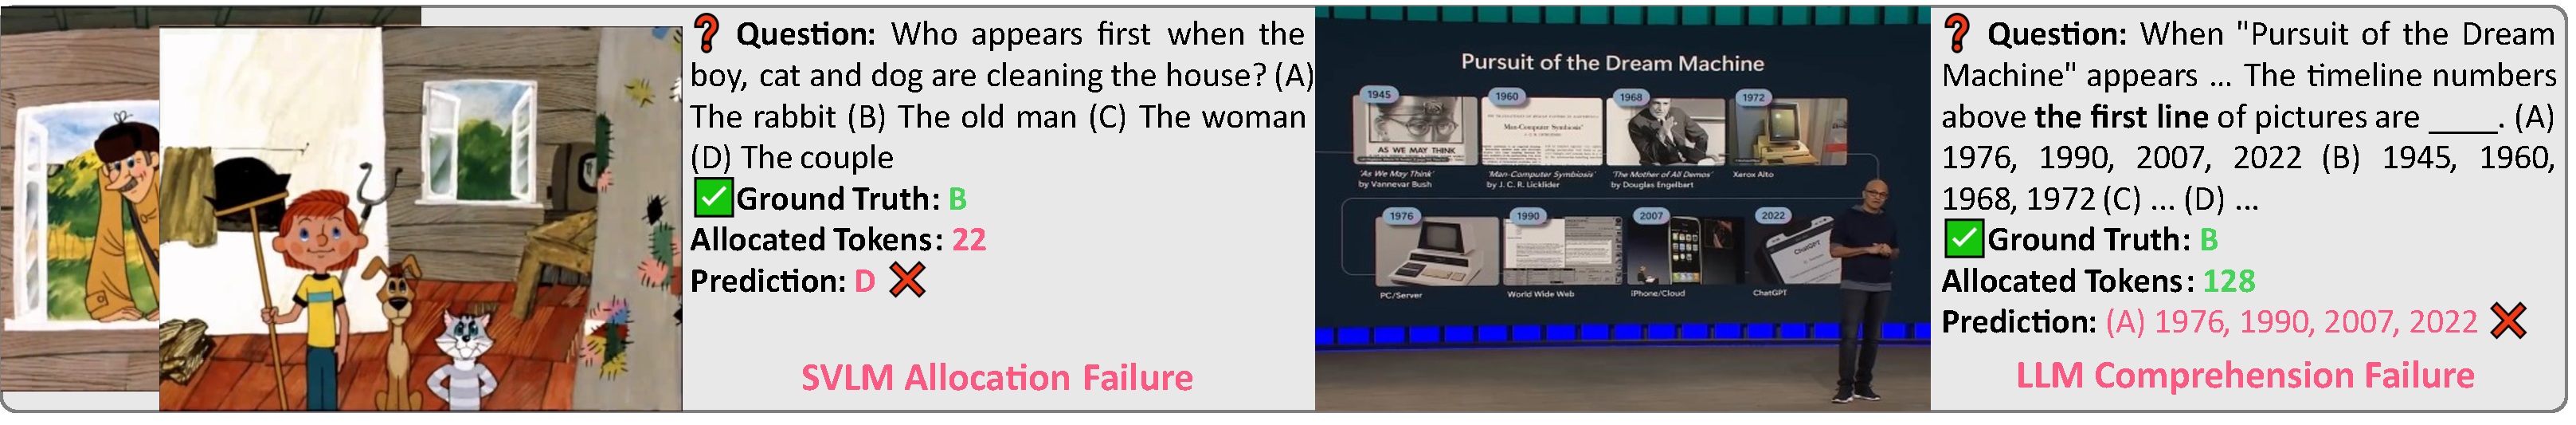
\includegraphics[width=0.44\textwidth]{fig/error.pdf}
    \vspace{-2em}
\end{figure}

%-------------------------------------------------------------------------
% References

% {
%     \small
%     \bibliographystyle{splncs04}
%     \bibliography{main}
% }

\end{document}
